\chapter{System Analysis}
\section{Introduction}
SafeSurf is a production-grade, infrastructure-aware Machine Learning system explicitly designed for real-time phishing website detection \cite{ref1}. The system provides definitive, actionable intelligence (Safe/Phishing) by analyzing Uniform Resource Locators (URLs) subjected to a layered, deterministic, and probabilistic pipeline. 

The core of SafeSurf combines a fast deterministic pre-check (DNS Guard) with a robust Multi-Model Voting Classifier Ensemble and Natural Language Processing (NLP). The architecture leverages 111 distinct features spanning lexical structure, domain age, SSL certificate details, and DNS infrastructure information to achieve a highly accurate detection capability ($> 97\%$ accuracy). Users interact with the system via a standalone Visual Security Dashboard and a real-time protective browser extension.
\section{Use Cases \&  Actors}
\subsection{Actors}
\begin{enumerate}
    \item \textbf{End User / Web Surfer:} The primary consumer of the system. They browse the internet and rely on the SafeSurf system to protect them from malicious websites. They interact with the system primarily through the Chrome extension and the web dashboard \cite{ref15}.
    \item \textbf{System Administrator / Security Analyst}: Responsible for managing the deployed application, monitoring real-time performance metrics via the dashboard, configuring .env thresholds, and actively re-training the ML models with updated datasets.
    \item \textbf{SafeSurf API (System Actor):} The FastAPI backend system that processes incoming requests, orchestrates the layered detection pipeline, interfaces with the ML models, and returns unified JSON risk analysis responses \cite{ref10}.
    \item \textbf{External Infrastructure (System Actors):} Third-party services, including DNS Resolvers, WHOIS registry databases, and SSL authorities. The system queries these actors to accumulate infrastructure footprint data for a given URL.
\end{enumerate}

\begin{figure}[H]
\centering
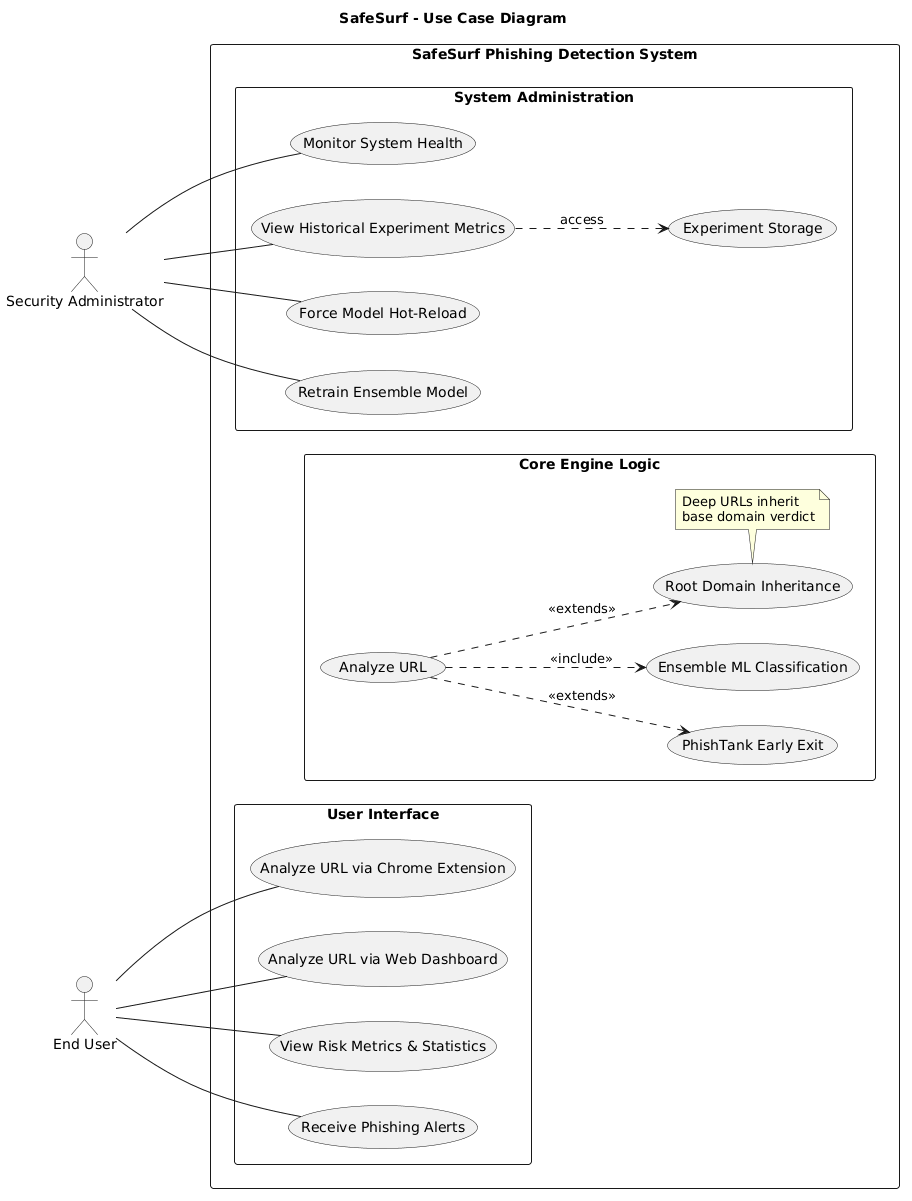
\includegraphics[width=0.8\textwidth]{./images/use-case-diagram.png}
\caption{System Use Case Diagram}
\label{fig:use_case}
\end{figure}

\subsection{Core Use Cases}
\begin{enumerate}
    \item \textbf{Analyze URL Safety:}
    An End User inputs a URL manually (or automatically via the extension). The system processes the URL and returns a definitive "safe", "phishing", or "invalid" verdict, mapping it to a risk level (LOW/MEDIUM/HIGH).

    \item \textbf{Model Re-training \& Evaluation:}
    The System Analyst utilizes the three-phase data pipeline to extract features from a raw CSV dataset, retrain the multi-model ensemble, and hot-reload the .pkl files into the live detection server without downtime.
    
    \item \textbf{Metric Dashboarding:}
    The End User or Analyst logs onto the web interface to view the system's historical detection accuracy rate, precision metrics, and ROC-AUC visualizations directly extracted from the metrics.json file.
    \item \textbf{Automated Browser Protection:}
    The Chrome Extension passively captures URLs visited by the End User, querying the API in the background. If a threshold is exceeded, it alerts or blocks the user from proceeding to the malicious site.
    
    \begin{figure}[H]
    \centering
    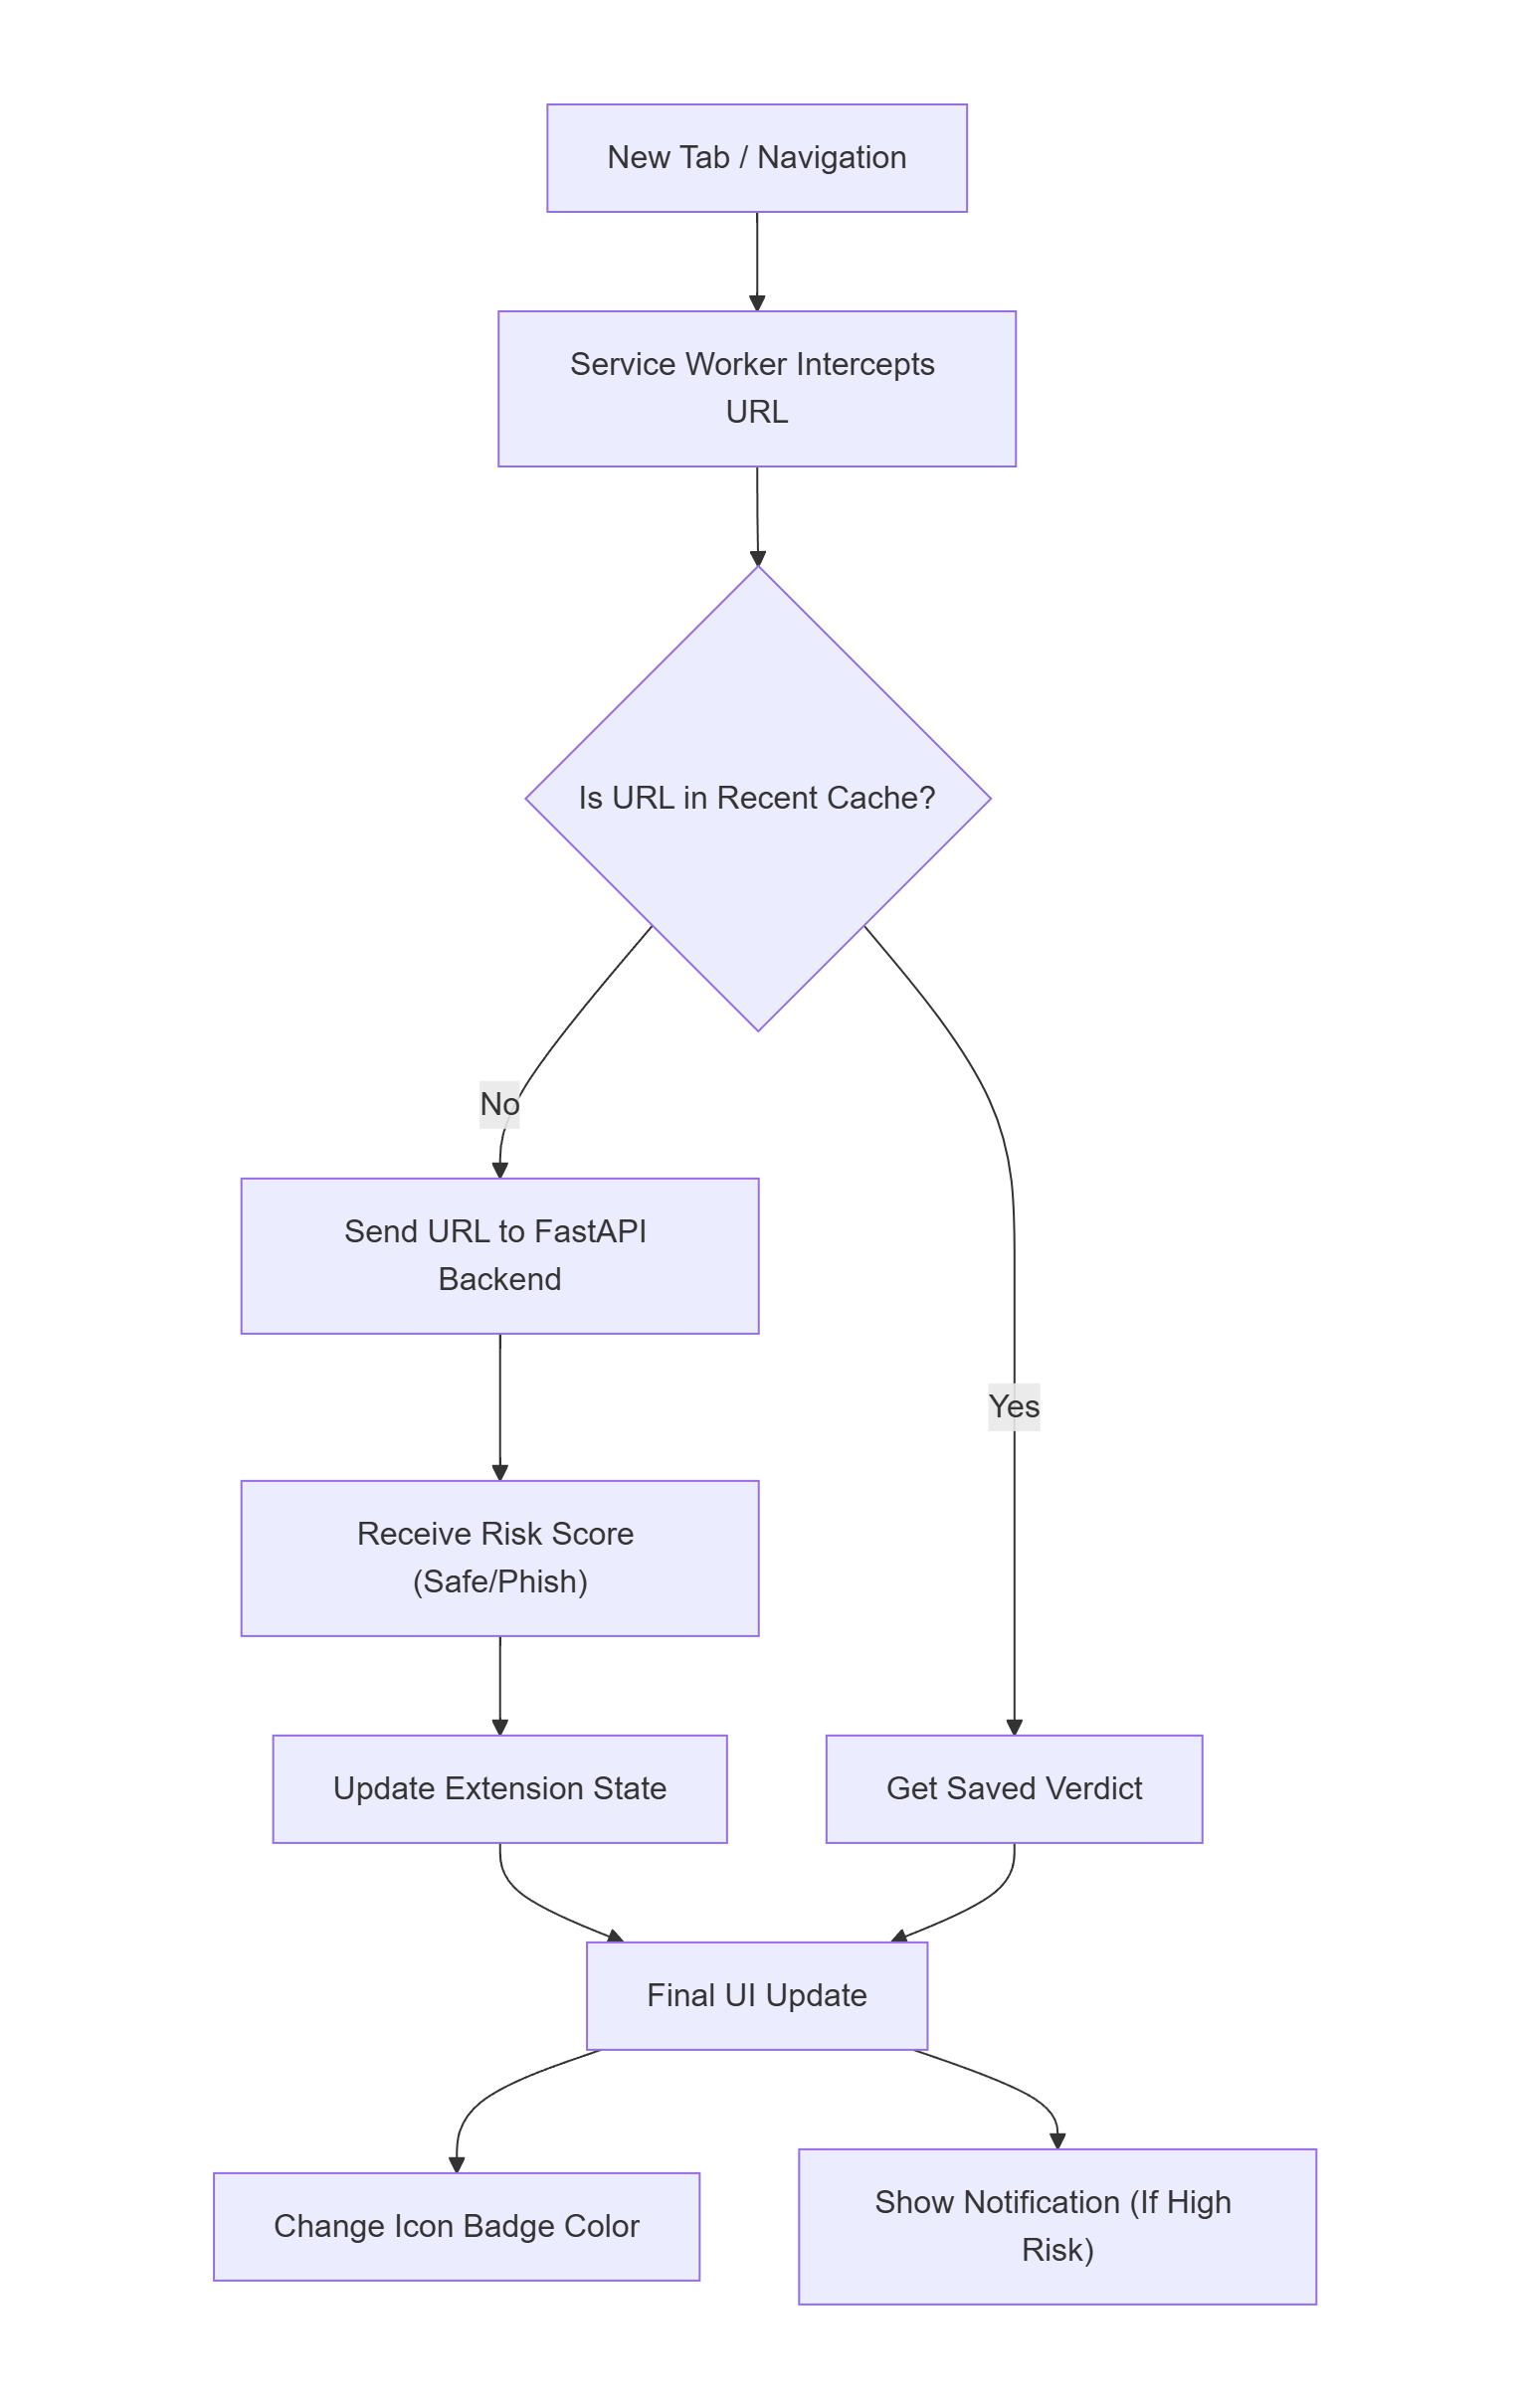
\includegraphics[width=0.7\textwidth]{./images/chrome-extension.png}
    \caption{Chrome Extension Real-Time Workflow}
    \label{fig:chrome_extension_flow}
    \end{figure}
\end{enumerate}

\section{Algorithms Used}
The detection engine utilizes a hybrid approach, merging deterministic heuristics with probabilistic machine learning models \cite{ref16}.

\subsection{DNS Guard (Deterministic DNS Resolution)}
\noindent
A pre-check algorithm ensuring the URL actually exists. It attempts to resolve the domain's A-record. If it returns NXDOMAIN (No Answer), the algorithm halts the pipeline and instantly flags the URL as "invalid" (High Risk), significantly saving computational resources.

\begin{figure}[H]
\centering
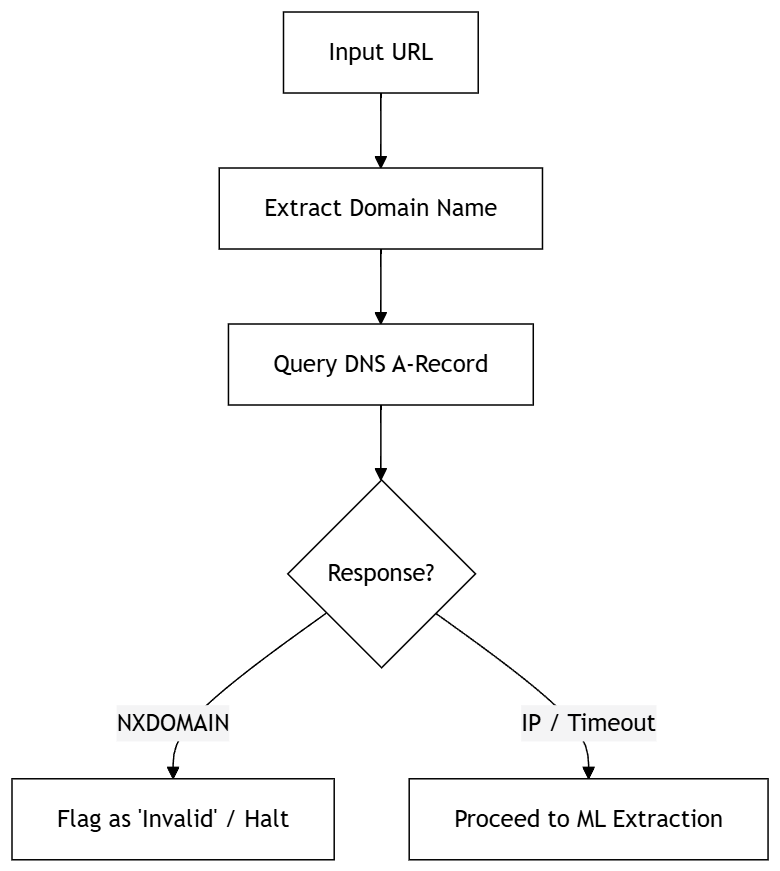
\includegraphics[width=0.5\textwidth]{./images/dns.png}
\caption{DNS Guard}
\label{fig:dns}
\end{figure}

\subsection{Multi-Model Voting Classifier Ensemble}
\noindent
A robust ensemble algorithm utilized for scikit-learn compatibility and overall generalization \cite{ref11}. It analyzes 111 deep structural features (character counts, DNS TTL, SSL properties, WHOIS timing) derived from comprehensive phishing datasets \cite{ref5}. The Voting Classifier internally aggregates predictions from:
\begin{itemize}
    \item Logistic Regression
    \item Linear Support Vector Classifier (LinearSVC)
    \item Random Forest Classifier
    \item Histogram-based Gradient Boosting Classifier
    \item eXtreme Gradient Boosting (XGBoost) \cite{ref12, ref13}
\end{itemize}

\begin{figure}[H]
\centering
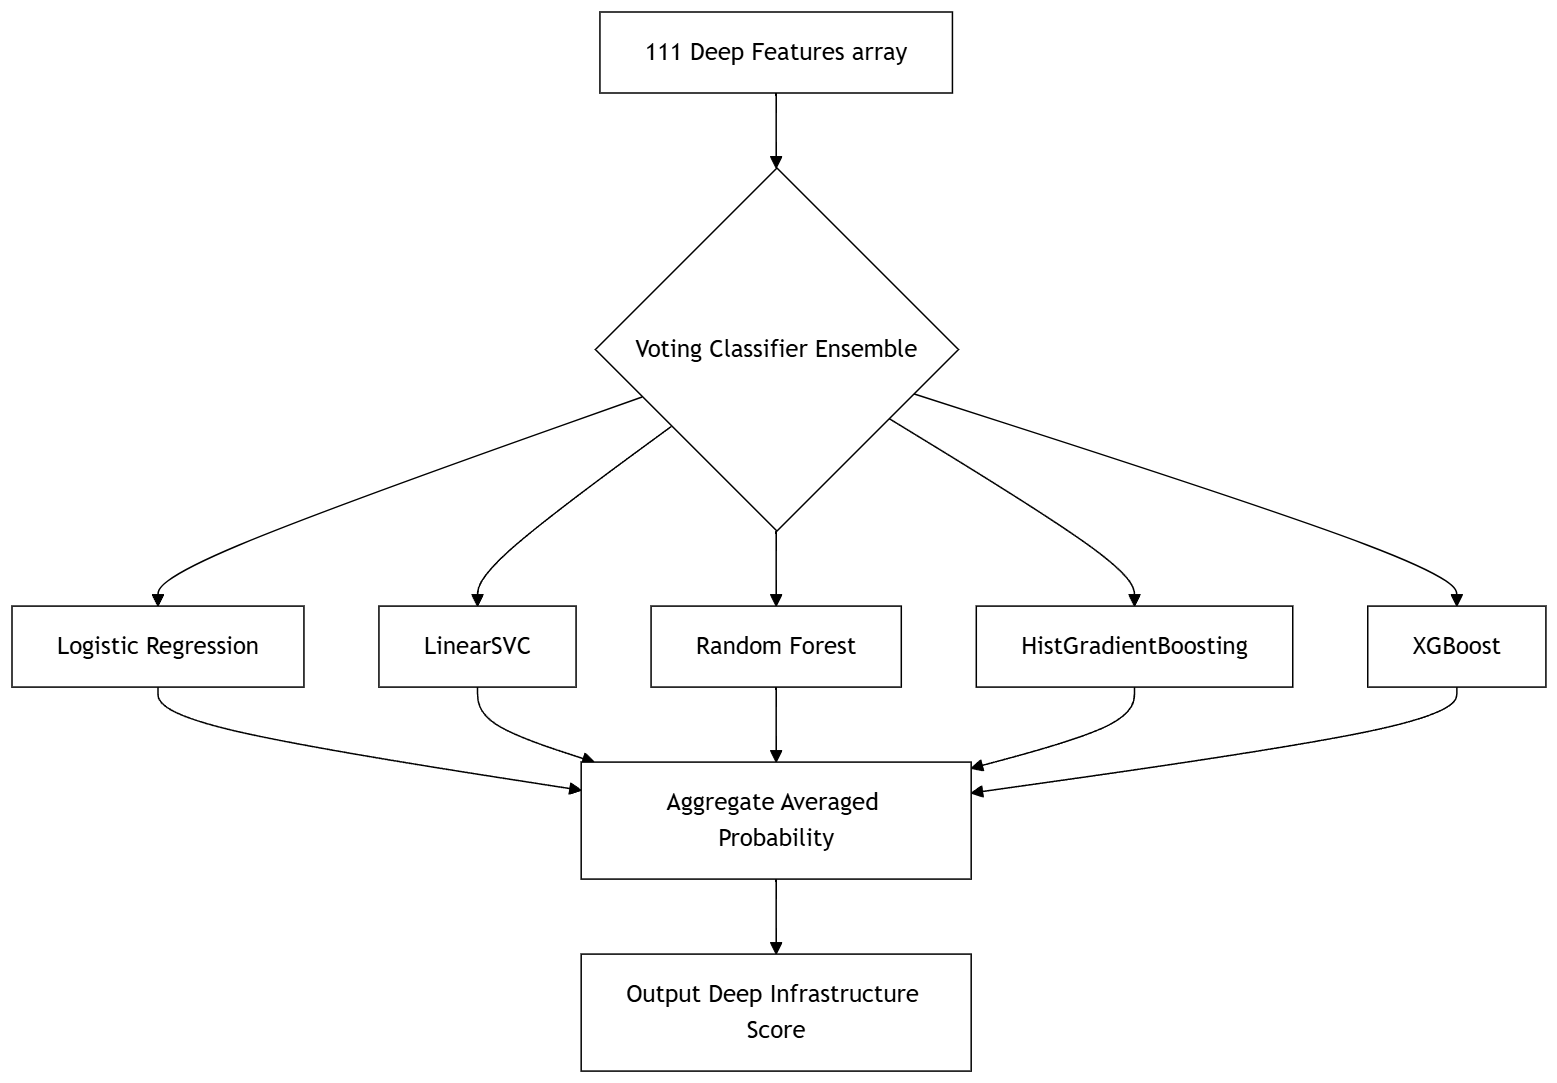
\includegraphics[width=0.70\textwidth]{./images/multi-model-voting.png}
\caption{Multi-Model Voting Classifier Ensemble}
\label{fig:multi-model}
\end{figure}

\subsection{Natural Language Processing - Bag of Words}
\noindent
An algorithm focusing solely on the lexical shape and text strings within the URL. It utilizes a CountVectorizer \cite{ref11} to generate token arrays and scores the visual characteristics using a LogisticRegression model.


\begin{figure}[H]
\centering
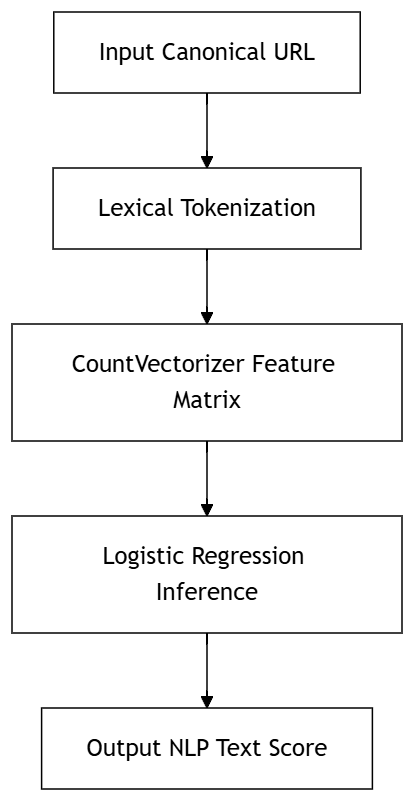
\includegraphics[width=0.3\textwidth]{./images/nlp.png}
\caption{Natural Language Processing}
\label{fig:nlp}
\end{figure}

\subsection{Weighted Soft-Voting Merger (Fusion Algorithm)}
\noindent
The overarching algorithm that merges the predictions from the Deep Infrastructure model and the NLP Text model. It computes a mathematically weighted probability to form the final verdict.

$\text{Final Probability} = (0.65 \times \text{XGB\_Ensemble\_Score}) + (0.35 \times \text{NLP\_Score})$

\begin{figure}[H]
\centering
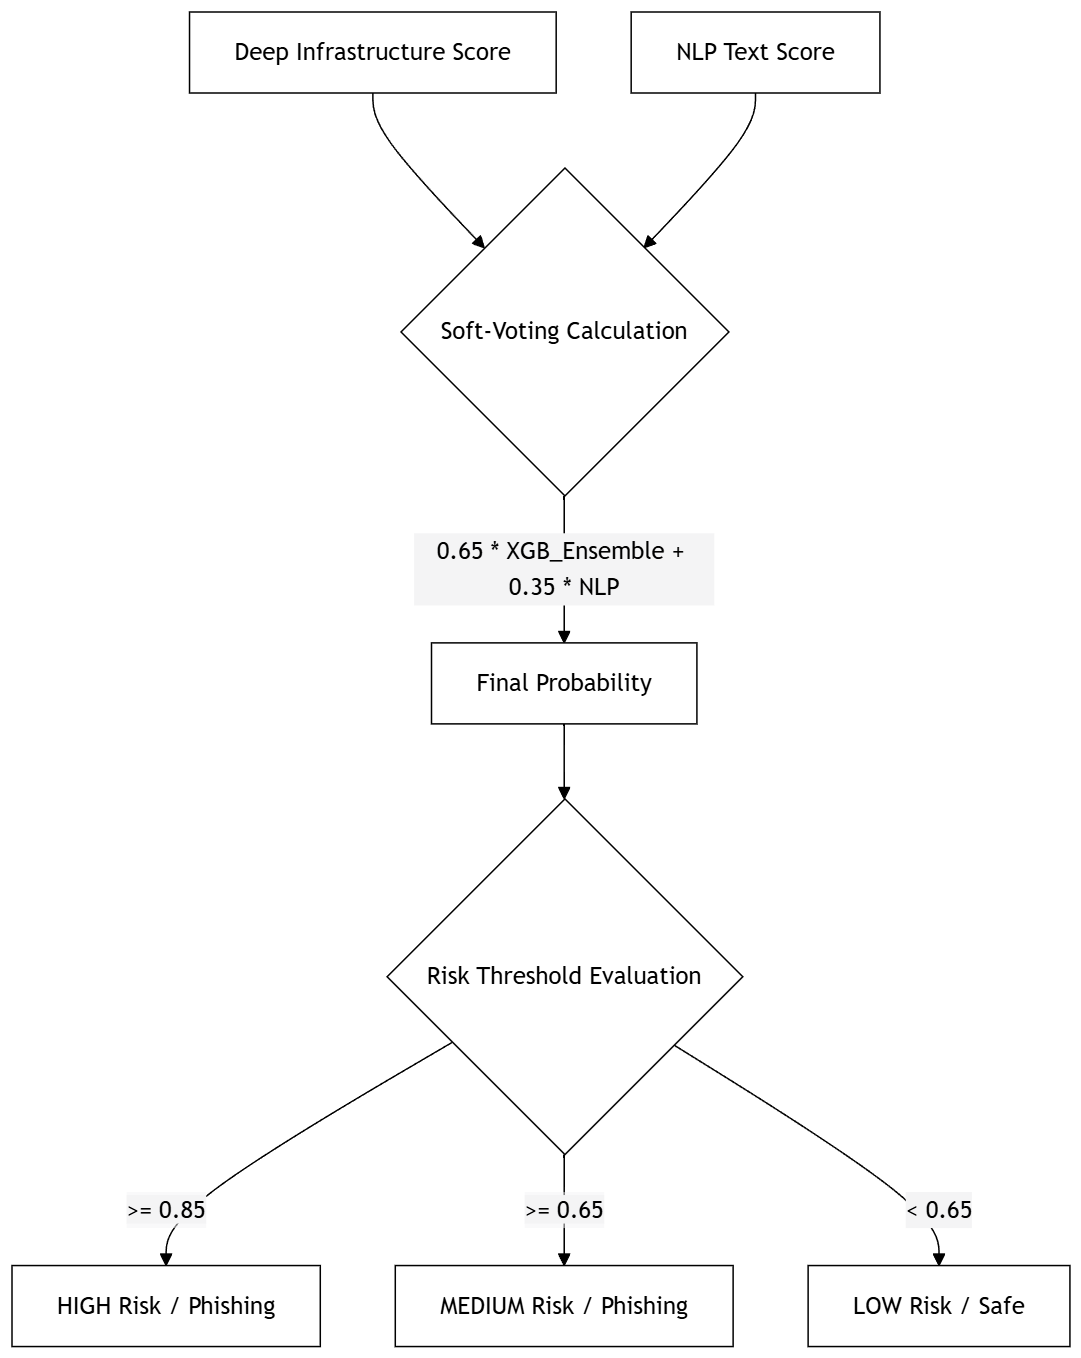
\includegraphics[width=0.5\textwidth]{./images/weighted-soft-voting.png}
\caption{Weighted Soft-Voting Merger}
\label{fig:weighted-soft-voting}
\end{figure}

\section{System Flow Chart}
The following flowchart illustrates the step-by-step pipeline from URL ingestion to the final risk classification.
\begin{figure}[H]
\centering
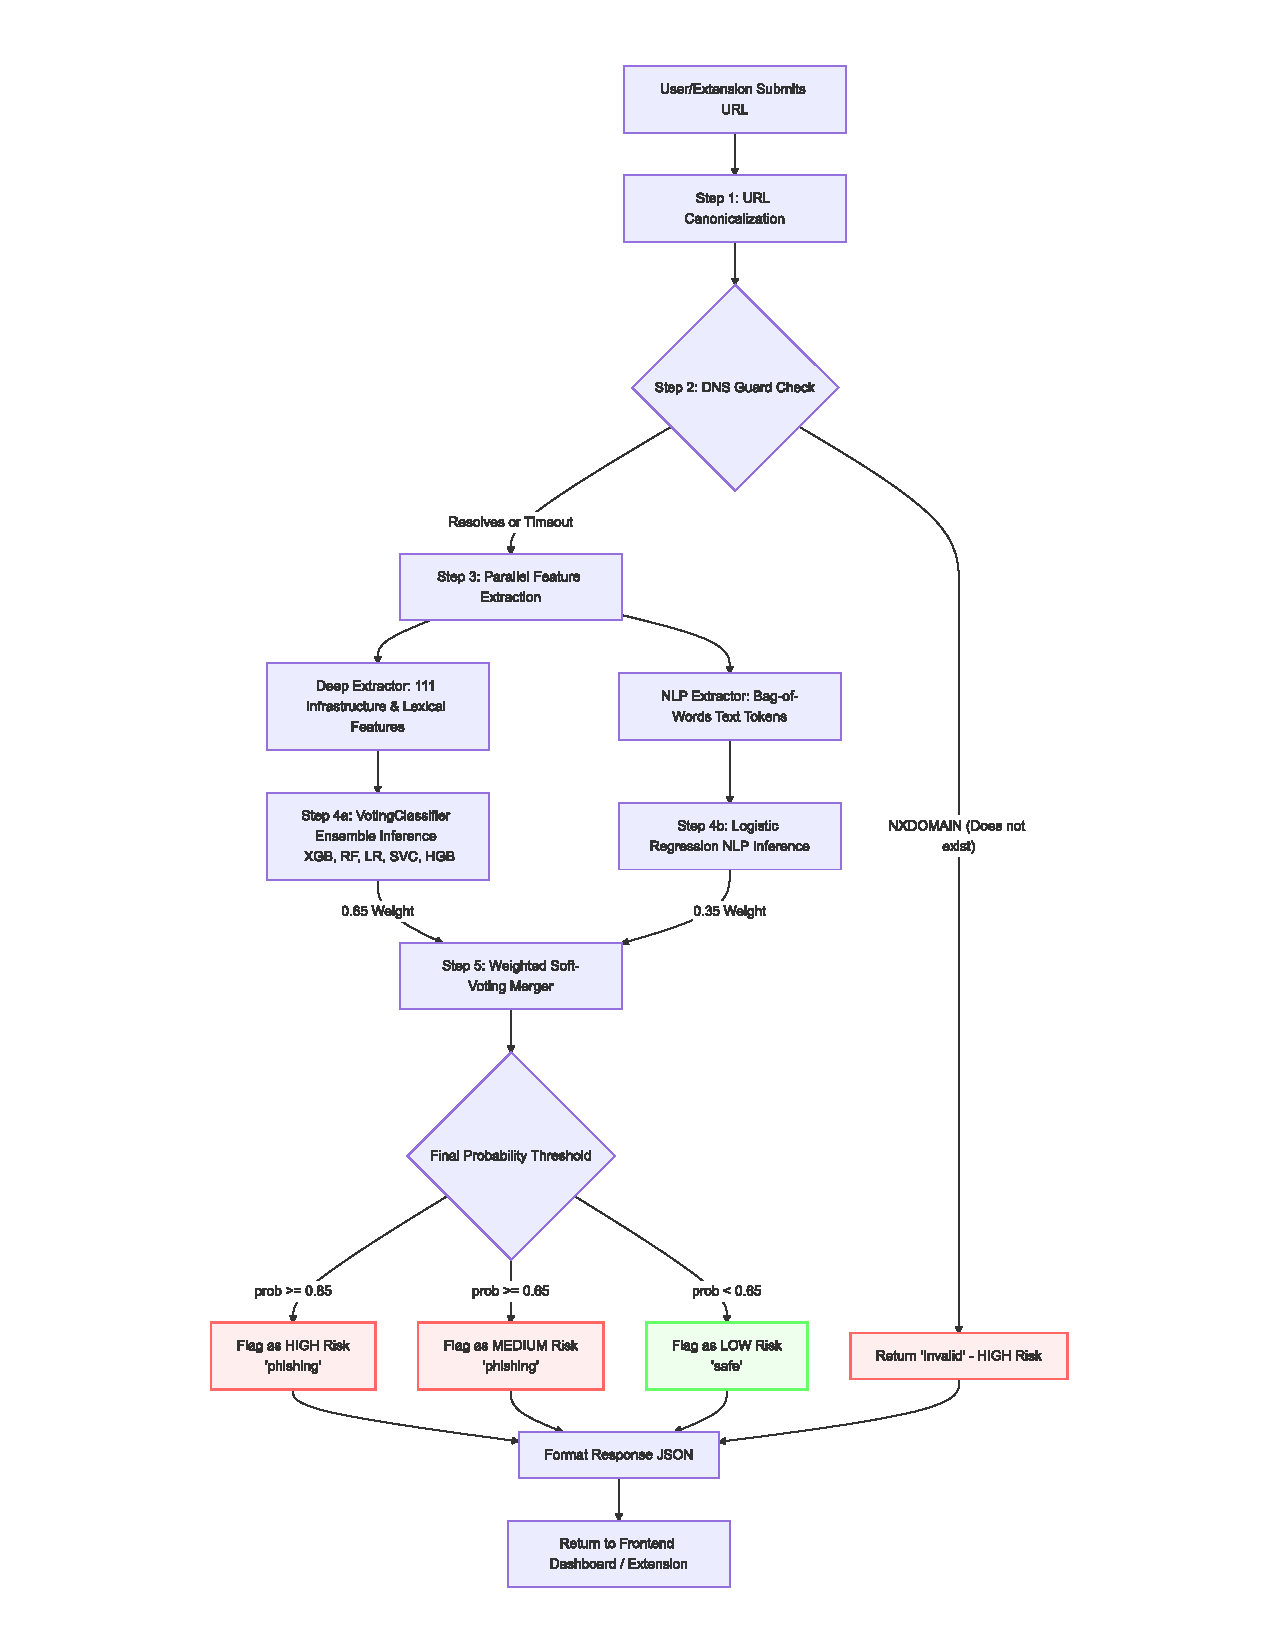
\includegraphics[width=\textwidth]{./images/flowchart.pdf}
\caption{System Flowchart}
\label{fig:flowchart}
\end{figure}
